% Name: Consumer and producer surplus
% Description: The market for one good at equilibrium: consumer surplus is the triangle under demand and above the price, producer surplus the triangle above supply and below it.
% Tags: consumer surplus, producer surplus, equilibrium, welfare, microeconomics

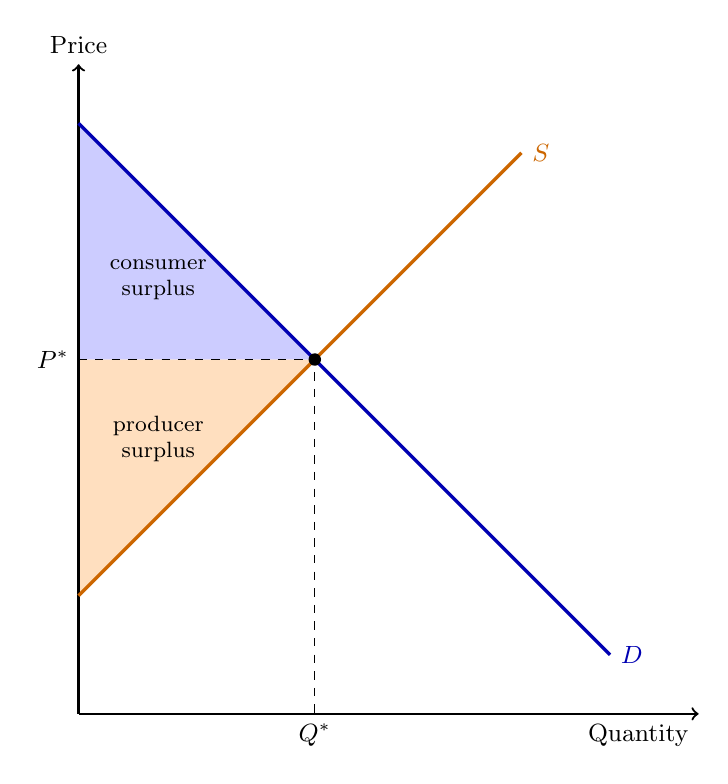
\begin{tikzpicture}[scale=0.75, every node/.style={font=\small}]
  % Demand P = 10 - Q and supply P = 2 + Q meet at Q* = 4, P* = 6
  \fill[blue!20] (0,10) -- (0,6) -- (4,6) -- cycle;
  \fill[orange!25] (0,6) -- (0,2) -- (4,6) -- cycle;
  \draw[->, thick] (0,0) -- (10.5,0) node[below left] {Quantity};
  \draw[->, thick] (0,0) -- (0,11) node[above] {Price};
  \draw[very thick, blue!70!black] (0,10) -- (9,1) node[right] {$D$};
  \draw[very thick, orange!80!black] (0,2) -- (7.5,9.5) node[right] {$S$};
  \draw[dashed] (0,6) node[left] {$P^*$} -| (4,0) node[below] {$Q^*$};
  \fill (4,6) circle (3pt);
  \node[align=center, font=\footnotesize] at (1.35,7.35) {consumer\\surplus};
  \node[align=center, font=\footnotesize] at (1.35,4.65) {producer\\surplus};
\end{tikzpicture}
